\chapter{Проектирование и реализация}

\section{Программная модель планировщика}

Ранее было выделено две основные сущности, из которых состоит проектируемый интеллектуальный агент: планирующий и диалоговый агенты. Целесообразно выделить в отдельный компонент обход плана в ходе его выполнения и алгоритмы выбора действий и вопросов. Тогда эта алгоритмическая база может быть в дальнейшем использована в множестве различных реализаций функциональности диалога.

Еще одна часть системы возникает из необходимости преобразования описаний предметной области из текстовой формы языка PDDL во внутреннее программное представление. Кроме того, предполагается, что в будущем будет возможно изменение этого представления с помощью диалогового агента.

\autoref{fig:archped} отображает взаимодействие этих компонентов.

\begin{figure}[H]
 \centering

 \begin{tikzpicture}[->,>=stealth', every node/.style={rectangle, draw},grow=right,auto,node distance=3cm]
  \node (import) {PDDL import};
  \node (planner) [right of=import] {Planner};
  \node (executor) [right of=planner] {Executor};
  \node (agent) [right of=executor] {Dialog agent};
  \path
    (import) edge[<->] (planner)
    (planner) edge[<->] (executor)
    (executor) edge[<->] (agent);
 \end{tikzpicture}

 \caption{Общая схема работы программной реализации агента}
 \label{fig:archped}
\end{figure}

\autoref{fig:process} описывает процесс достижения цели.

\begin{figure}[H]
 \centering
 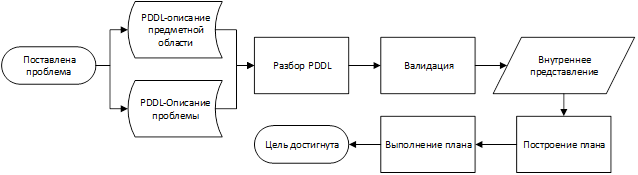
\includegraphics{process1.png}
 \caption{Блок-схема процесса достижения цели}
 \label{fig:process}
\end{figure}

\section{Инструментальные средства}

Разработка проекта ведется на языках высокого уровня Scala, Java. Общий объем кодовой базы составляет порядка 2300 LOC\footnote{LOC -- lines of code}. Основная функциональность покрыта приблизительно 50 юнит-тестами, объем кода которых занимает около 450 LOC от общего.

\subsection{Scala}

В качестве основного средства разработки был выбран язык Scala -
мультипарадигмальный язык программирования, спроектированный кратким и
типобезопасным для простого и быстрого создания компонентного
программного обеспечения, сочетающий возможности функционального и
объектно-ориентированного программирования (Wikipedia, 2014).

\begin{itemize}
\item
  Мощная система статической типизации с поддержкой абстрактных типов
  данных: traits, типажи
\item
  Полная совместимость с Java на уровне байт-кода
  JVM\footnote{JVM -- Java Virtual Machine, виртуальная
  машина Java}
\item
  DSL\footnote{DSL -- Domain Specific Language} для работы с логическими формулами, повышающий читаемость и
  выразительность кода: \texttt{val exp = 'L iff 'B \& 'S}
\item
  Функциональная парадигма программирования позволяет писать
  потокобезопасный код с использованием неизменяемых объектов, выражать
  алгоритмы в краткой рекурсивной форме без потери
  производительности с помощью хвостовой рекурсии\footnote{Хвостовая рекурсия (англ. tail recursion) --  частный случай рекурсии, при котором любой рекурсивный вызов является последней операцией перед возвратом из функции.}
\item
  Простая модель многопоточности без непосредственного управления
  жизненным циклом потока на основе передачи сообщений, с помощью
  классов Actor.
\item
  Встроенный генератор грамматических парсеров, аналогичный Java-библиотеке ANTLR.
\end{itemize}

\subsection{Обзор библиотек}

Проект не использует проприетарных решений и полностью построен на программных библиотеках с открытым исходным кодом. Хотя текущая реализация по качеству далека от необходимого для использования где-либо кроме учебных задач, она опирается на проверенные решения, имеющие большой запас производительности:

\begin{itemize*}
 \item SAT4J
 \item JGraphT
 \item Swing
\end{itemize*}

Отдельно можно выделить структуры данных и алгоритмы пакета \lstinline{scala.*} -- стандартной библиотеки языка. Повсеместно используются реализации списков, множеств, хэш-таблиц. По умолчанию подключаются неизменяемые (immutable) версии. В будущем это позволит избежать ошибок многопоточности с одновременным изменением одного объекта из нескольких потоков и отменяет нужду в синхронизации. Тем не менее, такой подход требует больших затрат оперативной памяти.

\subsubsection{SAT4J}

Пакет \lstinline{org.sat4j.scala.*} предоставляет набор классов и функций для записи и вычисления пропозициональных логических формул в форме DSL. Основным же компонентом является решатель задачи выполнимости булевых формул (SAT), который находится в пакете \lstinline{org.sat4j.core.*}. Библиотека предоставляет два варианта его реализации: основной и облегченный, оба доступны через шаблон проектирования ``Фабрика'':

\begin{lstlisting}
 ISolver default = org.sat4j.minisat.SolverFactory.defaultSolver();
 ISolver light = org.sat4j.minisat.SolverFactory.lightSolver();
\end{lstlisting}

Последний предназначен для задач с числом формул порядка 100-1000. Интерфейс ISolver принимает логические формулы в формате Dimacs, который представляет собой набор массивов целых чисел, где номер - индекс соответствующей переменной, знак минус соответствует отрицанию. Далее, отдельный массив представляет собой дизъюнкцию входящих в него литералов, а все вместе они образуют конъюктивную нормальную форму.

Доступны классы для конвертирования в этот формат из других, например привычной записи логических формул с помощью литералов и операций над ними -- эта функциональность используется при импорте из PDDL.

\subsubsection{JGraphT}

Java-библиотека работы с графами. Используемый API - DirectedMultigraph и его стандартная реализация, DefaultDirectedMultigraph.

\subsubsection{Swing}

Библиотека для создания графического интерфейса для программ
на языке Java. Swing был разработан компанией Sun Microsystems. Он
содержит ряд графических компонентов (англ. widgets), таких как кнопки,
поля ввода, таблицы и т. д.

Примитивный графический интерфейс был создан с его использованием.

\subsection{Средства сборки, организация исходного кода}

Исходный код организован в типичную для Maven-проектов структуру директорий:

\begin{description}
 \item[\textbf{src/main/scala}]\hfill \\
 Исходный код программы 
 \item[src/main/resources]\hfill \\
 Описание предметной области на языке PDDL
 \item[src/test/scala]\hfill \\
 Юнит-тесты
 \item[src/test/resources]\hfill \\
 Частичные описания предметных областей, конфигурации нагрузочного тестирования
\end{description}

\paragraph{Классы разбиты в иерархию пакетов, которая явно отделяет внешние API от внутренних. Права доступа заданы соответствущим образом.}

Базовым является пакет \lstinline{com.glowingavenger.*}.

\begin{description}
 \item[com.glowingavenger.agent.*]\hfill \\
 Классы исполнения плана
 \item[com.glowingavenger.dialog.*] \hfill \\
 Примеры реализации диалога с помощью графического интерфейса пользователя
 \item[com.glowingavenger.plan.*] \hfill \\
 Планировщик
 \begin{description}
  \item[impl.*]
  Компоненты построения условного плана
  \item[importexport.*]
  Импорт и экспорт
  \item[model.*]
  Классы предметной области планировщика: состояния, действия
  \item[util.*]
  Утилиты для работы с описанными выше библиотеками
 \end{description}
\end{description}

Для сборки используется Maven и/или SBT\footnote{Simple Build Tool -- популярный инструмент в среде Scala.}. В качестве среды разработки -- Intellij IDEA, Eclipse.

\begin{comment}
\section{Подходы, примененные в разработке}


\begin{lstlisting}[caption=LogicAction]
class LogicAction (
val precond: BoolExp,
val effect: BoolExp,
actionName: String) extends Action
\end{lstlisting}

\begin{lstlisting}[caption=Question]
case class Question(attr: Symbol) extends Action
\end{lstlisting}

\begin{lstlisting}[caption=NoAction]
case class NoAction() extends Action
\end{lstlisting}

\subsection{Состояния}

\begin{lstlisting}[caption=BeliefState]
abstract class AbstractBeliefState[E](val predicates: Map[E, Option[Boolean]]) {
  def unknown: Iterable[Symbol]

  def known: Map[Symbol, Option[Boolean]]

  def toExpr: BoolExp
  ...
}
\end{lstlisting}

\begin{lstlisting}[caption=Answer]
case class Answer(
    override val predicates: Map[Symbol, Option[Boolean]],
    attr: Symbol
) extends BeliefState(predicates) {
  val yes = BeliefState(predicates ++ Map(attr -> Some(true)))
  val no = BeliefState(predicates ++ Map(attr -> Some(false)))
  ...
}
\end{lstlisting}
\end{comment}
